% Created by tikzDevice version 0.12.6 on 2025-04-02 10:21:43
% !TEX encoding = UTF-8 Unicode
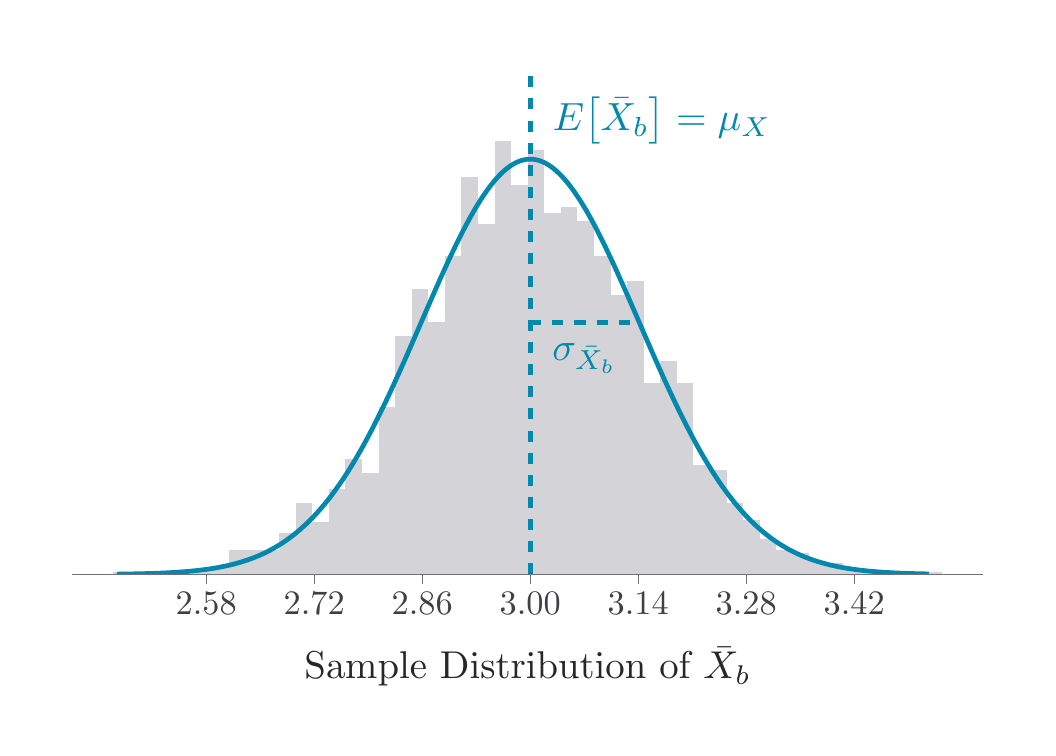
\begin{tikzpicture}[x=1pt,y=1pt]
\definecolor{fillColor}{RGB}{255,255,255}
\path[use as bounding box,fill=fillColor] (0,0) rectangle (361.35,252.94);
\begin{scope}
\path[clip] (  0.00,  0.00) rectangle (361.35,252.94);
\definecolor{drawColor}{RGB}{255,255,255}

\path[draw=drawColor,line width= 0.7pt,line join=round,line cap=round,fill=fillColor] (  0.00,  0.00) rectangle (361.35,252.94);
\end{scope}
\begin{scope}
\path[clip] ( 16.00, 55.37) rectangle (345.35,236.94);
\definecolor{drawColor}{RGB}{255,255,255}
\definecolor{fillColor}{RGB}{255,255,255}

\path[draw=drawColor,line width= 0.7pt,line join=round,line cap=round,fill=fillColor] ( 16.00, 55.37) rectangle (345.35,236.94);
\definecolor{fillColor}{RGB}{212,212,216}

\path[fill=fillColor] ( 30.97, 55.37) rectangle ( 36.96, 56.36);

\path[fill=fillColor] ( 36.96, 55.37) rectangle ( 42.95, 56.36);

\path[fill=fillColor] ( 42.95, 55.37) rectangle ( 48.94, 55.37);

\path[fill=fillColor] ( 48.94, 55.37) rectangle ( 54.92, 56.36);

\path[fill=fillColor] ( 54.92, 55.37) rectangle ( 60.91, 56.36);

\path[fill=fillColor] ( 60.91, 55.37) rectangle ( 66.90, 57.35);

\path[fill=fillColor] ( 66.90, 55.37) rectangle ( 72.89, 58.34);

\path[fill=fillColor] ( 72.89, 55.37) rectangle ( 78.88, 64.28);

\path[fill=fillColor] ( 78.88, 55.37) rectangle ( 84.86, 64.28);

\path[fill=fillColor] ( 84.86, 55.37) rectangle ( 90.85, 64.28);

\path[fill=fillColor] ( 90.85, 55.37) rectangle ( 96.84, 70.22);

\path[fill=fillColor] ( 96.84, 55.37) rectangle (102.83, 81.12);

\path[fill=fillColor] (102.83, 55.37) rectangle (108.82, 74.19);

\path[fill=fillColor] (108.82, 55.37) rectangle (114.81, 86.07);

\path[fill=fillColor] (114.81, 55.37) rectangle (120.79, 96.97);

\path[fill=fillColor] (120.79, 55.37) rectangle (126.78, 92.02);

\path[fill=fillColor] (126.78, 55.37) rectangle (132.77,115.79);

\path[fill=fillColor] (132.77, 55.37) rectangle (138.76,141.54);

\path[fill=fillColor] (138.76, 55.37) rectangle (144.75,158.38);

\path[fill=fillColor] (144.75, 55.37) rectangle (150.73,146.50);

\path[fill=fillColor] (150.73, 55.37) rectangle (156.72,170.27);

\path[fill=fillColor] (156.72, 55.37) rectangle (162.71,198.99);

\path[fill=fillColor] (162.71, 55.37) rectangle (168.70,182.16);

\path[fill=fillColor] (168.70, 55.37) rectangle (174.69,211.87);

\path[fill=fillColor] (174.69, 55.37) rectangle (180.68,196.02);

\path[fill=fillColor] (180.68, 55.37) rectangle (186.66,208.90);

\path[fill=fillColor] (186.66, 55.37) rectangle (192.65,186.12);

\path[fill=fillColor] (192.65, 55.37) rectangle (198.64,188.10);

\path[fill=fillColor] (198.64, 55.37) rectangle (204.63,183.15);

\path[fill=fillColor] (204.63, 55.37) rectangle (210.62,170.27);

\path[fill=fillColor] (210.62, 55.37) rectangle (216.60,156.40);

\path[fill=fillColor] (216.60, 55.37) rectangle (222.59,161.35);

\path[fill=fillColor] (222.59, 55.37) rectangle (228.58,124.70);

\path[fill=fillColor] (228.58, 55.37) rectangle (234.57,132.63);

\path[fill=fillColor] (234.57, 55.37) rectangle (240.56,124.70);

\path[fill=fillColor] (240.56, 55.37) rectangle (246.54, 94.99);

\path[fill=fillColor] (246.54, 55.37) rectangle (252.53, 93.01);

\path[fill=fillColor] (252.53, 55.37) rectangle (258.52, 81.12);

\path[fill=fillColor] (258.52, 55.37) rectangle (264.51, 75.18);

\path[fill=fillColor] (264.51, 55.37) rectangle (270.50, 68.24);

\path[fill=fillColor] (270.50, 55.37) rectangle (276.49, 64.28);

\path[fill=fillColor] (276.49, 55.37) rectangle (282.47, 63.29);

\path[fill=fillColor] (282.47, 55.37) rectangle (288.46, 60.32);

\path[fill=fillColor] (288.46, 55.37) rectangle (294.45, 59.33);

\path[fill=fillColor] (294.45, 55.37) rectangle (300.44, 57.35);

\path[fill=fillColor] (300.44, 55.37) rectangle (306.43, 56.36);

\path[fill=fillColor] (306.43, 55.37) rectangle (312.42, 55.37);

\path[fill=fillColor] (312.41, 55.37) rectangle (318.40, 56.36);

\path[fill=fillColor] (318.40, 55.37) rectangle (324.39, 55.37);

\path[fill=fillColor] (324.39, 55.37) rectangle (330.38, 56.36);
\definecolor{drawColor}{RGB}{1,136,172}

\path[draw=drawColor,line width= 1.7pt,line join=round] ( 32.21, 55.48) --
	( 33.19, 55.49) --
	( 34.18, 55.50) --
	( 35.16, 55.52) --
	( 36.14, 55.53) --
	( 37.12, 55.55) --
	( 38.10, 55.57) --
	( 39.08, 55.59) --
	( 40.06, 55.61) --
	( 41.05, 55.63) --
	( 42.03, 55.65) --
	( 43.01, 55.68) --
	( 43.99, 55.71) --
	( 44.97, 55.74) --
	( 45.95, 55.77) --
	( 46.93, 55.81) --
	( 47.92, 55.85) --
	( 48.90, 55.89) --
	( 49.88, 55.93) --
	( 50.86, 55.98) --
	( 51.84, 56.03) --
	( 52.82, 56.09) --
	( 53.80, 56.15) --
	( 54.78, 56.22) --
	( 55.77, 56.29) --
	( 56.75, 56.36) --
	( 57.73, 56.45) --
	( 58.71, 56.53) --
	( 59.69, 56.63) --
	( 60.67, 56.73) --
	( 61.65, 56.83) --
	( 62.64, 56.95) --
	( 63.62, 57.07) --
	( 64.60, 57.20) --
	( 65.58, 57.34) --
	( 66.56, 57.49) --
	( 67.54, 57.65) --
	( 68.52, 57.82) --
	( 69.50, 58.00) --
	( 70.49, 58.20) --
	( 71.47, 58.40) --
	( 72.45, 58.62) --
	( 73.43, 58.85) --
	( 74.41, 59.09) --
	( 75.39, 59.35) --
	( 76.37, 59.63) --
	( 77.36, 59.92) --
	( 78.34, 60.23) --
	( 79.32, 60.55) --
	( 80.30, 60.90) --
	( 81.28, 61.26) --
	( 82.26, 61.64) --
	( 83.24, 62.05) --
	( 84.22, 62.47) --
	( 85.21, 62.92) --
	( 86.19, 63.39) --
	( 87.17, 63.89) --
	( 88.15, 64.41) --
	( 89.13, 64.96) --
	( 90.11, 65.53) --
	( 91.09, 66.13) --
	( 92.08, 66.76) --
	( 93.06, 67.42) --
	( 94.04, 68.11) --
	( 95.02, 68.83) --
	( 96.00, 69.58) --
	( 96.98, 70.37) --
	( 97.96, 71.19) --
	( 98.94, 72.04) --
	( 99.93, 72.93) --
	(100.91, 73.85) --
	(101.89, 74.81) --
	(102.87, 75.81) --
	(103.85, 76.84) --
	(104.83, 77.92) --
	(105.81, 79.03) --
	(106.80, 80.18) --
	(107.78, 81.37) --
	(108.76, 82.60) --
	(109.74, 83.88) --
	(110.72, 85.19) --
	(111.70, 86.55) --
	(112.68, 87.94) --
	(113.66, 89.38) --
	(114.65, 90.86) --
	(115.63, 92.38) --
	(116.61, 93.94) --
	(117.59, 95.55) --
	(118.57, 97.19) --
	(119.55, 98.88) --
	(120.53,100.60) --
	(121.52,102.36) --
	(122.50,104.16) --
	(123.48,106.00) --
	(124.46,107.88) --
	(125.44,109.79) --
	(126.42,111.74) --
	(127.40,113.72) --
	(128.39,115.73) --
	(129.37,117.78) --
	(130.35,119.85) --
	(131.33,121.95) --
	(132.31,124.07) --
	(133.29,126.22) --
	(134.27,128.39) --
	(135.25,130.59) --
	(136.24,132.79) --
	(137.22,135.02) --
	(138.20,137.26) --
	(139.18,139.51) --
	(140.16,141.76) --
	(141.14,144.02) --
	(142.12,146.29) --
	(143.11,148.56) --
	(144.09,150.82) --
	(145.07,153.07) --
	(146.05,155.32) --
	(147.03,157.56) --
	(148.01,159.78) --
	(148.99,161.99) --
	(149.97,164.17) --
	(150.96,166.33) --
	(151.94,168.46) --
	(152.92,170.56) --
	(153.90,172.63) --
	(154.88,174.66) --
	(155.86,176.65) --
	(156.84,178.60) --
	(157.83,180.50) --
	(158.81,182.36) --
	(159.79,184.16) --
	(160.77,185.90) --
	(161.75,187.59) --
	(162.73,189.21) --
	(163.71,190.77) --
	(164.69,192.27) --
	(165.68,193.69) --
	(166.66,195.05) --
	(167.64,196.33) --
	(168.62,197.53) --
	(169.60,198.65) --
	(170.58,199.70) --
	(171.56,200.66) --
	(172.55,201.54) --
	(173.53,202.33) --
	(174.51,203.03) --
	(175.49,203.65) --
	(176.47,204.17) --
	(177.45,204.61) --
	(178.43,204.95) --
	(179.41,205.20) --
	(180.40,205.36) --
	(181.38,205.43) --
	(182.36,205.40) --
	(183.34,205.28) --
	(184.32,205.07) --
	(185.30,204.77) --
	(186.28,204.37) --
	(187.27,203.88) --
	(188.25,203.31) --
	(189.23,202.64) --
	(190.21,201.88) --
	(191.19,201.04) --
	(192.17,200.12) --
	(193.15,199.11) --
	(194.13,198.02) --
	(195.12,196.85) --
	(196.10,195.60) --
	(197.08,194.28) --
	(198.06,192.89) --
	(199.04,191.42) --
	(200.02,189.89) --
	(201.00,188.29) --
	(201.99,186.63) --
	(202.97,184.91) --
	(203.95,183.13) --
	(204.93,181.30) --
	(205.91,179.42) --
	(206.89,177.49) --
	(207.87,175.52) --
	(208.85,173.50) --
	(209.84,171.45) --
	(210.82,169.36) --
	(211.80,167.24) --
	(212.78,165.10) --
	(213.76,162.92) --
	(214.74,160.73) --
	(215.72,158.51) --
	(216.71,156.28) --
	(217.69,154.04) --
	(218.67,151.78) --
	(219.65,149.52) --
	(220.63,147.26) --
	(221.61,144.99) --
	(222.59,142.73) --
	(223.58,140.47) --
	(224.56,138.22) --
	(225.54,135.97) --
	(226.52,133.74) --
	(227.50,131.53) --
	(228.48,129.33) --
	(229.46,127.15) --
	(230.44,124.99) --
	(231.43,122.85) --
	(232.41,120.74) --
	(233.39,118.66) --
	(234.37,116.60) --
	(235.35,114.58) --
	(236.33,112.58) --
	(237.31,110.62) --
	(238.30,108.69) --
	(239.28,106.80) --
	(240.26,104.95) --
	(241.24,103.13) --
	(242.22,101.35) --
	(243.20, 99.61) --
	(244.18, 97.91) --
	(245.16, 96.24) --
	(246.15, 94.62) --
	(247.13, 93.04) --
	(248.11, 91.51) --
	(249.09, 90.01) --
	(250.07, 88.55) --
	(251.05, 87.14) --
	(252.03, 85.76) --
	(253.02, 84.43) --
	(254.00, 83.14) --
	(254.98, 81.89) --
	(255.96, 80.68) --
	(256.94, 79.52) --
	(257.92, 78.39) --
	(258.90, 77.30) --
	(259.88, 76.24) --
	(260.87, 75.23) --
	(261.85, 74.26) --
	(262.83, 73.32) --
	(263.81, 72.41) --
	(264.79, 71.55) --
	(265.77, 70.71) --
	(266.75, 69.91) --
	(267.74, 69.15) --
	(268.72, 68.41) --
	(269.70, 67.71) --
	(270.68, 67.04) --
	(271.66, 66.40) --
	(272.64, 65.79) --
	(273.62, 65.20) --
	(274.60, 64.64) --
	(275.59, 64.11) --
	(276.57, 63.60) --
	(277.55, 63.12) --
	(278.53, 62.66) --
	(279.51, 62.23) --
	(280.49, 61.81) --
	(281.47, 61.42) --
	(282.46, 61.05) --
	(283.44, 60.70) --
	(284.42, 60.36) --
	(285.40, 60.05) --
	(286.38, 59.75) --
	(287.36, 59.47) --
	(288.34, 59.20) --
	(289.32, 58.95) --
	(290.31, 58.71) --
	(291.29, 58.49) --
	(292.27, 58.28) --
	(293.25, 58.08) --
	(294.23, 57.90) --
	(295.21, 57.72) --
	(296.19, 57.56) --
	(297.18, 57.41) --
	(298.16, 57.26) --
	(299.14, 57.13) --
	(300.12, 57.00) --
	(301.10, 56.88) --
	(302.08, 56.77) --
	(303.06, 56.67) --
	(304.05, 56.57) --
	(305.03, 56.48) --
	(306.01, 56.40) --
	(306.99, 56.32) --
	(307.97, 56.25) --
	(308.95, 56.18) --
	(309.93, 56.12) --
	(310.91, 56.06) --
	(311.90, 56.00) --
	(312.88, 55.95) --
	(313.86, 55.91) --
	(314.84, 55.86) --
	(315.82, 55.82) --
	(316.80, 55.79) --
	(317.78, 55.75) --
	(318.77, 55.72) --
	(319.75, 55.69) --
	(320.73, 55.66) --
	(321.71, 55.64) --
	(322.69, 55.61) --
	(323.67, 55.59) --
	(324.65, 55.57) --
	(325.63, 55.56);

\path[draw=drawColor,line width= 1.7pt,dash pattern=on 4pt off 4pt ,line join=round] (181.59, 55.37) -- (181.59,236.94);

\path[] (188.10,211.49) --
	(268.74,211.49) --
	(268.64,211.49) --
	(269.05,211.51) --
	(269.46,211.59) --
	(269.84,211.73) --
	(270.20,211.94) --
	(270.52,212.20) --
	(270.80,212.51) --
	(271.02,212.86) --
	(271.18,213.24) --
	(271.28,213.64) --
	(271.31,214.06) --
	(271.31,214.06) --
	(271.31,226.82) --
	(271.31,226.82) --
	(271.28,227.23) --
	(271.18,227.63) --
	(271.02,228.01) --
	(270.80,228.36) --
	(270.52,228.67) --
	(270.20,228.93) --
	(269.84,229.14) --
	(269.46,229.29) --
	(269.05,229.37) --
	(268.74,229.39) --
	(188.10,229.39) --
	(188.41,229.37) --
	(188.00,229.39) --
	(187.59,229.34) --
	(187.19,229.22) --
	(186.81,229.04) --
	(186.47,228.81) --
	(186.18,228.52) --
	(185.93,228.19) --
	(185.73,227.83) --
	(185.60,227.43) --
	(185.54,227.03) --
	(185.53,226.82) --
	(185.53,214.06) --
	(185.54,214.26) --
	(185.54,213.85) --
	(185.60,213.44) --
	(185.73,213.05) --
	(185.93,212.68) --
	(186.18,212.35) --
	(186.47,212.07) --
	(186.81,211.83) --
	(187.19,211.65) --
	(187.59,211.54) --
	(188.00,211.49) --
	cycle;
\end{scope}
\begin{scope}
\path[clip] ( 16.00, 55.37) rectangle (345.35,236.94);
\definecolor{drawColor}{RGB}{1,136,172}

\node[text=drawColor,anchor=base west,inner sep=0pt, outer sep=0pt, scale=  1.42] at (189.81,215.77) {$\mathbb{E}\big[\bar{X}_b\big] = \mu_{X}$};
\end{scope}
\begin{scope}
\path[clip] ( 16.00, 55.37) rectangle (345.35,236.94);
\definecolor{drawColor}{RGB}{1,136,172}

\path[draw=drawColor,line width= 1.7pt,dash pattern=on 4pt off 4pt ,line join=round] (181.59,146.39) -- (221.01,146.39);

\path[] (187.89,128.48) --
	(214.71,128.48) --
	(214.60,128.48) --
	(215.02,128.50) --
	(215.42,128.58) --
	(215.81,128.73) --
	(216.17,128.94) --
	(216.49,129.20) --
	(216.76,129.51) --
	(216.98,129.86) --
	(217.15,130.24) --
	(217.24,130.64) --
	(217.28,131.05) --
	(217.28,131.05) --
	(217.28,143.82) --
	(217.28,143.82) --
	(217.24,144.23) --
	(217.15,144.63) --
	(216.98,145.01) --
	(216.76,145.36) --
	(216.49,145.67) --
	(216.17,145.93) --
	(215.81,146.14) --
	(215.42,146.28) --
	(215.02,146.37) --
	(214.71,146.39) --
	(187.89,146.39) --
	(188.20,146.37) --
	(187.78,146.38) --
	(187.37,146.33) --
	(186.98,146.22) --
	(186.60,146.04) --
	(186.26,145.81) --
	(185.96,145.52) --
	(185.72,145.19) --
	(185.52,144.82) --
	(185.39,144.43) --
	(185.33,144.02) --
	(185.32,143.82) --
	(185.32,131.05) --
	(185.33,131.26) --
	(185.33,130.85) --
	(185.39,130.44) --
	(185.52,130.05) --
	(185.72,129.68) --
	(185.96,129.35) --
	(186.26,129.06) --
	(186.60,128.83) --
	(186.98,128.65) --
	(187.37,128.53) --
	(187.78,128.48) --
	cycle;
\end{scope}
\begin{scope}
\path[clip] ( 16.00, 55.37) rectangle (345.35,236.94);
\definecolor{drawColor}{RGB}{1,136,172}

\node[text=drawColor,anchor=base,inner sep=0pt, outer sep=0pt, scale=  1.42] at (201.30,132.77) {$\sigma_{\bar{X}_b}$};
\end{scope}
\begin{scope}
\path[clip] (  0.00,  0.00) rectangle (361.35,252.94);
\definecolor{drawColor}{RGB}{113,113,122}

\path[draw=drawColor,line width= 0.3pt,line join=round] ( 16.00, 55.37) --
	(345.35, 55.37);
\end{scope}
\begin{scope}
\path[clip] (  0.00,  0.00) rectangle (361.35,252.94);
\definecolor{drawColor}{RGB}{113,113,122}

\path[draw=drawColor,line width= 0.3pt,line join=round] ( 64.51, 51.87) --
	( 64.51, 55.37);

\path[draw=drawColor,line width= 0.3pt,line join=round] (103.54, 51.87) --
	(103.54, 55.37);

\path[draw=drawColor,line width= 0.3pt,line join=round] (142.56, 51.87) --
	(142.56, 55.37);

\path[draw=drawColor,line width= 0.3pt,line join=round] (181.59, 51.87) --
	(181.59, 55.37);

\path[draw=drawColor,line width= 0.3pt,line join=round] (220.61, 51.87) --
	(220.61, 55.37);

\path[draw=drawColor,line width= 0.3pt,line join=round] (259.64, 51.87) --
	(259.64, 55.37);

\path[draw=drawColor,line width= 0.3pt,line join=round] (298.66, 51.87) --
	(298.66, 55.37);
\end{scope}
\begin{scope}
\path[clip] (  0.00,  0.00) rectangle (361.35,252.94);
\definecolor{drawColor}{RGB}{63,63,70}

\node[text=drawColor,anchor=base,inner sep=0pt, outer sep=0pt, scale=  1.24] at ( 64.51, 40.91) {2.58};

\node[text=drawColor,anchor=base,inner sep=0pt, outer sep=0pt, scale=  1.24] at (103.54, 40.91) {2.72};

\node[text=drawColor,anchor=base,inner sep=0pt, outer sep=0pt, scale=  1.24] at (142.56, 40.91) {2.86};

\node[text=drawColor,anchor=base,inner sep=0pt, outer sep=0pt, scale=  1.24] at (181.59, 40.91) {3.00};

\node[text=drawColor,anchor=base,inner sep=0pt, outer sep=0pt, scale=  1.24] at (220.61, 40.91) {3.14};

\node[text=drawColor,anchor=base,inner sep=0pt, outer sep=0pt, scale=  1.24] at (259.64, 40.91) {3.28};

\node[text=drawColor,anchor=base,inner sep=0pt, outer sep=0pt, scale=  1.24] at (298.66, 40.91) {3.42};
\end{scope}
\begin{scope}
\path[clip] (  0.00,  0.00) rectangle (361.35,252.94);
\definecolor{drawColor}{RGB}{39,39,42}

\node[text=drawColor,anchor=base,inner sep=0pt, outer sep=0pt, scale=  1.40] at (180.68, 17.65) {Sample Distribution of $\bar{X}_b$};
\end{scope}
\end{tikzpicture}
